\begin{frame}
    \centering
    \begin{figure}[H]
        
\includegraphics[keepaspectratio, width=0.7\paperwidth, height=\paperheight]{LeeLogo}
    \end{figure}
    Informatik: Programmieren\\
    \textbf{Feedback zu Übungen}\emoji{nerd-face}
\end{frame}


\begin{frame}[fragile]{Lektion 08}
\tib{Aufgabe 3.38} (Reiskörner): Was könnte hier besser gemacht werden?
\begin{lstlisting}[style=TigerJython]
def summe(anzahl, zahl):
    resultat = 0
    repeat anzahl:
        print(zahl, resultat)
        resultat += zahl
        zahl*= 2
    print(resultat)
    
summe(63, 1)
\end{lstlisting}
\begin{itemize}
    \item Zeile 1: sind \pythoninline{resultat} und \pythoninline{zahl} gute Variablennamen?
    \item Zeile 2: weshalb \pythoninline{resultat=0}?
\end{itemize}
\end{frame}

\begin{frame}[fragile]{Lektion 09}
\tib{Aufgabe 3.40} (Wort $10\cdot 10$ mal drucken): Was könnte hier besser gemacht werden?
\begin{lstlisting}[style=TigerJython]
from gturtle import*

makeTurtle()
def druckewort(anzahl):
    wort = input("Welche Zahl?")
    repeat(anzahl):
        print(wort*10)
        
druckewort(10)
\end{lstlisting}
\begin{itemize}
    \item Zeilen 1-3: Weshalb \pythoninline{from gturtle import*} und \pythoninline{makeTurtle()}?
    \item Zeile 4: Weshalb \pythoninline{def}?
    \item Zeile 5: Weshalb \pythoninline{input("Welche Zahl")}?
\end{itemize}
\end{frame}


\begin{frame}[fragile]{Lektion 10}
\tib{Aufgabe 4.11}: Was könnte hier besser gemacht werden?\\[-.5cm]
\begin{minipage}[t]{.45\textwidth}
    \begin{lstlisting}[style=TigerJython, basicstyle=\tiny]
from gturtle import*
def vieleck(ecken,seite,farbe):
    setPenColor(farbe)
    repeat ecken:
        forward(seite)
        right(360/ecken)
def vieleck_sicher(zahl):
    if zahl ==1:
        vieleck(4,50,"red")
    if zahl ==2:
        vieleck(3,50,"green")
    
        
    if zahl ==3:
        vieleck(6,50,"blue")
        
    else:
        print("Nur 1/2/3 gehen!")

makeTurtle()
zahl =input("Zahl 1-10")
vieleck_sicher(zahl)
\end{lstlisting}
\end{minipage}
\begin{minipage}[t]{.45\textwidth}
    \begin{lstlisting}[style=TigerJython, basicstyle=\tiny, showstringspaces=false]
from gturtle import *

def vieleck(ecken, seite, farbe):
    setPenColor(farbe)
    repeat ecken:
        forward(seite)
        right(360/ecken)
        
def vieleck_sicher(zahl):
    if zahl==1:
        vieleck(4, 50, "red")
    if zahl==2:
        vieleck(3, 50, "green")
    if zahl==3:
        vieleck(6, 50, "blue")
    else:
        print("Nur 1/2/3 gehen!")

makeTurtle()
zahl=input("Zahl 1-10")
vieleck_sicher(zahl)
\end{lstlisting}
\end{minipage}
\begin{minipage}[c]{.45\textwidth}
    \begin{itemize}
        \item Finde die 10 Unterschiede...
    \end{itemize}
\end{minipage}
\begin{minipage}[c]{.48\textwidth}
    \begin{figure}[H]
    \centering
    
\includegraphics[keepaspectratio, width=.25\paperwidth, height=\paperheight]{GrundlagenInfo/Programmieren/Figures/prog-make_it_nice.jpeg}
    \end{figure}
\end{minipage}
\end{frame}

\begin{frame}[fragile]{Lektion 10}
\tib{Aufgabe 4.11}: Was könnte hier besser gemacht werden?\\[-.5cm]
\begin{minipage}[t]{.45\textwidth}
    \begin{lstlisting}[style=TigerJython, basicstyle=\tiny]
from gturtle import *

def vieleck(ecken, seite, farbe):
    setPenColor(farbe)
    repeat ecken:
        forward(seite)
        right(360/ecken)
        
def vieleck_sicher(zahl):
    if zahl==1:
        vieleck(4,50, "red")
    if zahl==2:
        vieleck(3,50, "green")
    if zahl==3:
        vieleck(6,50, "blue")
    else:
        print("Nur 1/2/3 gehen!")

makeTurtle()
zahl=input("Zahl 1-10")
vieleck_sicher(zahl)
\end{lstlisting}
\end{minipage}
\begin{minipage}[t]{.45\textwidth}
    \begin{lstlisting}[style=TigerJython, basicstyle=\tiny]
from gturtle import *

def vieleck(ecken, farbe):
    setPenColor(farbe)
    repeat ecken:
        forward(50)
        right(360/ecken)
        
def vieleck_sicher(zahl):
    if zahl==1:
        vieleck(4, "red")
    if zahl==2:
        vieleck(3, "green")
    if zahl==3:
        vieleck(6, "blue")
    else:
        print("Nur 1/2/3 gehen!")

makeTurtle()
zahl=input("Zahl 1-10")
vieleck_sicher(zahl)
\end{lstlisting}
\end{minipage}
\begin{minipage}[c]{.3\textwidth}
    \begin{figure}[H]
    \centering
    
\includegraphics[keepaspectratio, width=.25\paperwidth, height=\paperheight]{GrundlagenInfo/Programmieren/Figures/prog-make_it_nice.jpeg}
    \end{figure}
\end{minipage}
\begin{minipage}[c]{.66\textwidth}
    \begin{itemize}
        \item ... \& make it simple!
        \item Ein Parameter, der immer den gleichen Wert annimmt, kann als Konstante geschrieben werden
    \end{itemize}
\end{minipage}
\end{frame}


\begin{frame}[fragile]{Lektion 10}
\tib{Aufgabe 4.11}: Was könnte hier besser gemacht werden?\\[-.5cm]
\begin{minipage}[t]{.45\textwidth}
    \begin{lstlisting}[style=TigerJython, basicstyle=\tiny]
from gturtle import *

def vieleck(ecken, seite, farbe):
        
def vieleck_sicher(zahl):
    if zahl==1:
        setPenColor("red")
        repeat 4:
            forward(50)
            right(360/4)
    if zahl==2:
        setPenColor("red")
        repeat 3:
            forward(50)
            right(360/3)
    if zahl==3:
        setPenColor("green")
        repeat 6:
            forward(50)
            right(360/6)
    else:
        print("Nur 1/2/3 gehen!")

makeTurtle()
zahl=input("Zahl 1-10")
vieleck_sicher(zahl)
\end{lstlisting}
\end{minipage}
\begin{minipage}[t]{.45\textwidth}
    \begin{lstlisting}[style=TigerJython, basicstyle=\tiny]
from gturtle import *

def vieleck(ecken, farbe):
    setPenColor(farbe)
    repeat ecken:
        forward(50)
        right(360/ecken)
        
def vieleck_sicher(zahl):
    if zahl==1:
        vieleck(4, "red")
    if zahl==2:
        vieleck(3, "green")
    if zahl==3:
        vieleck(6, "blue")
    else:
        print("Nur 1/2/3 gehen!")

makeTurtle()
zahl=input("Zahl 1-10")
vieleck_sicher(zahl)
\end{lstlisting}
\end{minipage}
\begin{minipage}[c]{.48\textwidth}
    \begin{itemize}
        \item Code \tib{modularisieren}
    \end{itemize}
\end{minipage}
\begin{minipage}[c]{.48\textwidth}
    \begin{figure}[H]
        \centering
        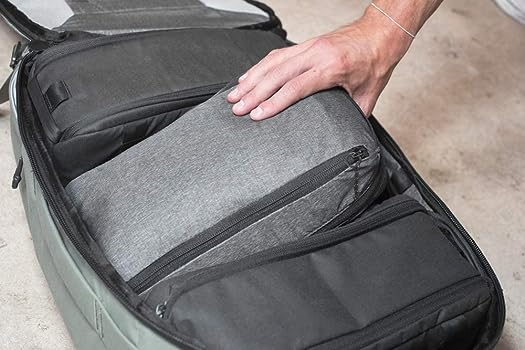
\includegraphics[keepaspectratio, width=.15\paperwidth]{GrundlagenInfo/Programmieren/Figures/prog-packing-cubes.jpg}
    \end{figure}
\end{minipage}
\end{frame}

\begin{frame}[fragile]{Lektion 10}
\tib{Aufgabe 4.11}: Was könnte hier besser gemacht werden?\\[-.5cm]
\begin{minipage}[t]{.45\textwidth}
    \begin{lstlisting}[style=TigerJython, basicstyle=\tiny]
from gturtle import*

def quadrat():
    repeat 4:
        forward(50)
        right(90)
        
def drehen():
    runden =input("Wie viele Runden soll das Quadrat machen?")
    repeat runden:
        repeat 360:
            setPenWidth(1)
            setPenColor("black")
            quadrat()
            delay(1)
            setPenWidth(10)
            setPenColor("white")
            quadrat()   
            right(1)
    
makeTurtle()
hideTurtle()
drehen()
\end{lstlisting}
\begin{figure}[H]
        \centering
        
\includegraphics[keepaspectratio, width=.13\paperwidth]{GrundlagenInfo/Programmieren/Figures/prog-comment.jpg}
    \end{figure}
\end{minipage}
\begin{minipage}[t]{.45\textwidth}
    \begin{lstlisting}[style=TigerJython, basicstyle=\tiny]
from gturtle import*

def quadrat():
    repeat 4:
        forward(50)
        right(90)
        
def drehen():
    runden =input("Wie viele Runden soll das Quadrat machen?")
    repeat runden:
        repeat 360:
            # quadrat malen
            setPenWidth(1)
            setPenColor("black")
            quadrat()
            delay(1) # 1 ms warten
            # quadrat auslöschen
            setPenWidth(10)
            setPenColor("white")
            quadrat()
            # nach rechts drehen
            right(1)
    
makeTurtle()
hideTurtle()
drehen()
\end{lstlisting}
\end{minipage}
\end{frame}

\begin{frame}{Code-Qualität \emoji{nerd-face}}{Zusammenfassung}
    Ein guter Code ist:
    \begin{itemize}
        \item möglichst \textbf{kurz und leserlich}
        \item \textbf{modular}, so dass man ihn einfach in Unterteile zerlegen kann
        \item schön und leserlich sowie \textbf{konsistent formatiert}
        \item gut dokumentiert mit \textbf{Kommentaren}
        \item \textbf{verständlich} und enthält \textbf{selbst-erklärende} Variablen- und Funktionen-Namen
    \end{itemize}
    \begin{figure}[H]
        \centering
        
\includegraphics[keepaspectratio, height=.15\paperheight]{GrundlagenInfo/Programmieren/Figures/prog-make_it_nice.jpeg}
        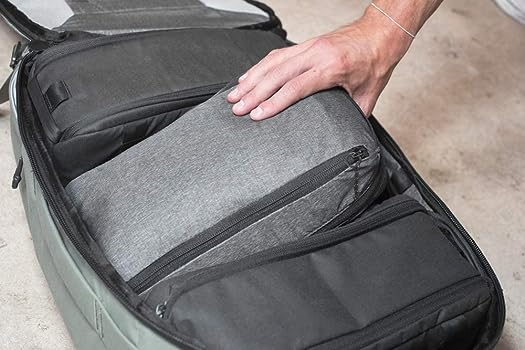
\includegraphics[keepaspectratio, height=.15\paperheight]{GrundlagenInfo/Programmieren/Figures/prog-packing-cubes.jpg}
        
\includegraphics[keepaspectratio, height=.15\paperheight]{GrundlagenInfo/Programmieren/Figures/prog-comment.jpg}
        
\includegraphics[keepaspectratio, height=.15\paperheight]{GrundlagenInfo/Programmieren/Figures/prog-confused.jpg}
    \end{figure}
\end{frame}




